\chapter{Поиск точек бифуркаций}

Найдя предельный цикл в системе \ref{lab:eq:2}, мы можем перейти к следующему
этапу нашего исследования -- определения всех значений параметра, при которых
наблюдается данный цикл.

В силу того, что наша система рассматривается дифференциальным уравнением,
поведение системы будет меняться плавно на промежутках, разделенных так
называемыми, точками \textit{бифуркации}(точки, в которых происходит изменение
поведения системы).

\begin{definition}
    Точка бифуркации - значение параметра системы, при котором наблюдается
    качественное изменение поведения системы.
\end{definition}

Чтобы нам было удобно наблюдать изменение системы от параметра без перезапуска
программы, мы обернем построения в функцию и добавим в нашу программу слайдер --
бегунок, которым можно будет менять значение параметра $\nu$.

\begin{figure}
    \centering
    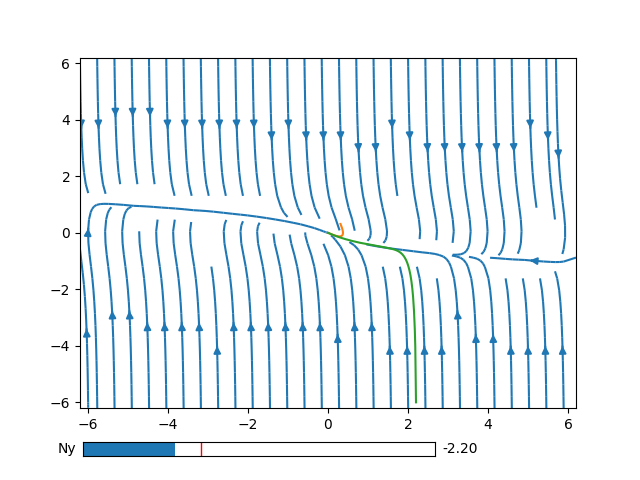
\includegraphics[width=0.8\textwidth]{figures/2_point_-2_2}
    \caption{Стационарная точка системы при $\nu = -2.2$}
    \label{lab2:point_-2}
\end{figure}

Начиная с отрицательных значений (от -10) мы наблюдаем сильное стремление
к центру координат -- стационарной точки системы (График \ref{lab2:point_-2}).

\begin{figure}[!ht]
    \centering
    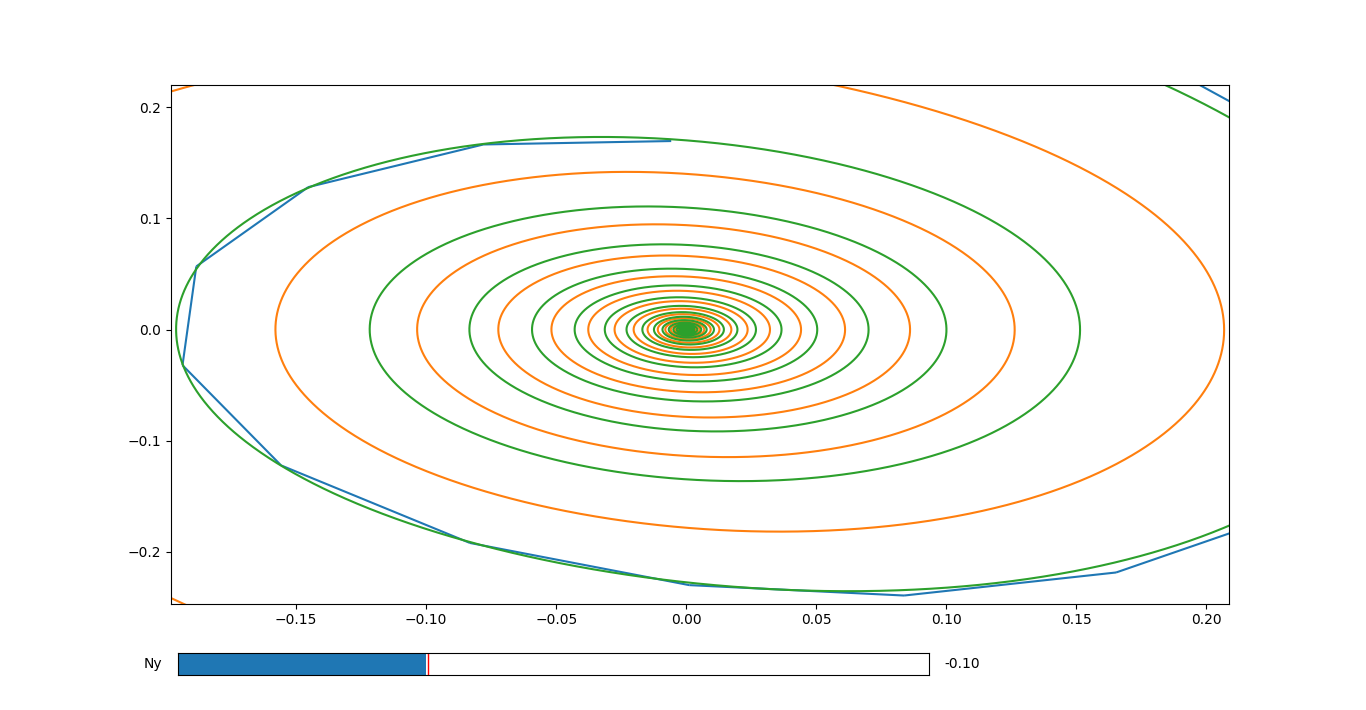
\includegraphics[width=0.8\textwidth]{figures/2_point_-0_1}
    \caption{Стационарная точка системы при $\nu = -0.1$}
    \label{lab2:point_0}
\end{figure}

При приближении параметра к нулю, поведение системы искривляется в овальную
форму, но линии медленно сходятся к нулю (График \ref{lab2:point_0}).

\begin{figure}[!ht]
    \centering
    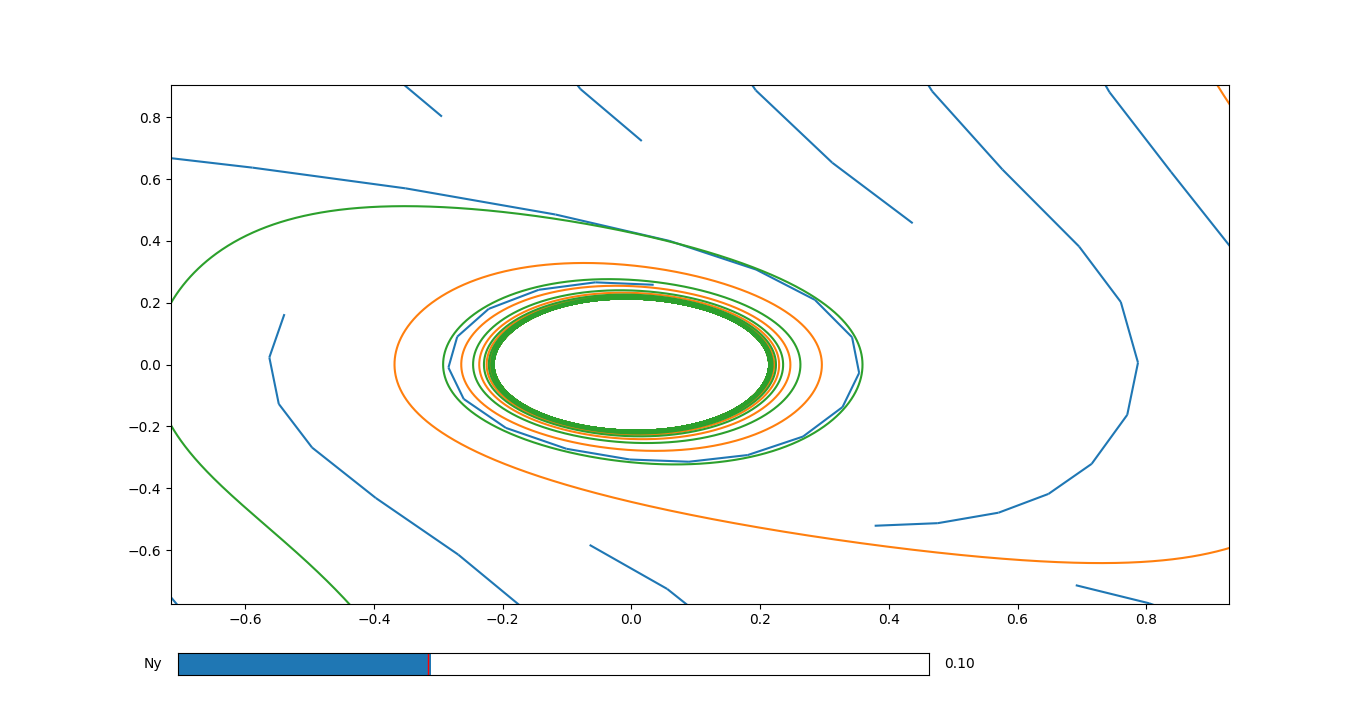
\includegraphics[width=0.8\textwidth]{figures/2_cycle_0_1}
    \caption{Появление цикла при $\nu = 0.1$}
    \label{lab2:cycle_0_1}
\end{figure}

Как только мы переступаем нулевое значение параметра, наши траектории
останавливаются значительно раньше -- мы начинаем наблюдать знакомый нам
предельный цикл, но в меньших размерах (График \ref{lab2:cycle_0_1}).

\begin{figure}[!ht]
    \centering
    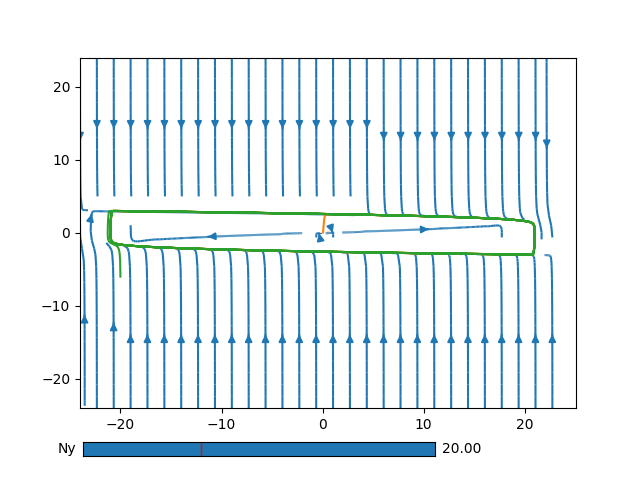
\includegraphics[width=0.8\textwidth]{figures/2_cycle_20}
    \caption{Расширение предельного цикла при увеличении параметра ($\nu = 20$)}
    \label{lab2:cycle_20}
\end{figure}

Увеличивая $\nu$ дальше, остается наблюдать за ростом цикла(График
\ref{lab2:cycle_20}).

Из полученных наблюдений можно выдвинуть гипотезу: на отрицательной полуоси
исследуемая система сходится в стационарную точку; в положительной же оси
наблюдается предельный цикл, который увеличивается в зависимости от параметра
системы.

Стоит отметить, что наличие или отсутствие предельного цикла на границе
($\nu = 0$) мы выявить не можем, так как при приближении к параметра к нулю,
чтобы быть уверенным в наличии стационарной точки или цикла, приходится
увеличивать точность вычислений. В конце концов, когда точность увеличить
не удается, нам остается только предполагать: толи линии сошлись к циклу, толи
они не достигли нуля из-за недостаточного кол-ва шагов в методе Эйлера.

С учетом этого замечания, можно выдвинуть еще одну гипотезу: так как изменение
поведения в системе происходит настолько плавно, что нам не удается уловить
момент, когда точка мы наблюдаем стационарную точку, а когда предельный цикл,
то мы можем сказать, что наблюдается \textit{мягкая бифуркация системы}.
